\documentclass{ctexart}
    \usepackage{mathrsfs}
    \usepackage{multirow}
    \usepackage{graphicx}
    \usepackage{array}
    \usepackage{makecell}
    \usepackage{amsmath}
    \usepackage{booktabs}
    \usepackage{float}
    \usepackage{diagbox}
    \newcommand\mgape[1]{\gape{$\vcenter{\hbox{#1}}$}}
    \newcommand\Ronum[1]{\uppercase\expandafter{\romannumeral #1\relax}}
    \newcommand\ronum[1]{\romannumeral #1\relax}
    \author{钱思天\ 1600011388 No.7}
    \title{实验二十\ 光衍射的定量研究 \ 实验报告}
    \begin{document}
      \maketitle
      \section{单缝、多缝缝宽及缝间隔计算}
      \subsection{单缝}
      \subsubsection{实验数据图}
      选用编号为$
      \uppercase\expandafter{\romannumeral3}4(\mbox{缝宽参考值为}133\mu m)$经过测量,并运用数据分析软件,得图如下:
      \begin{figure}[H]
        \centering
        \caption{单缝衍射结果图}
        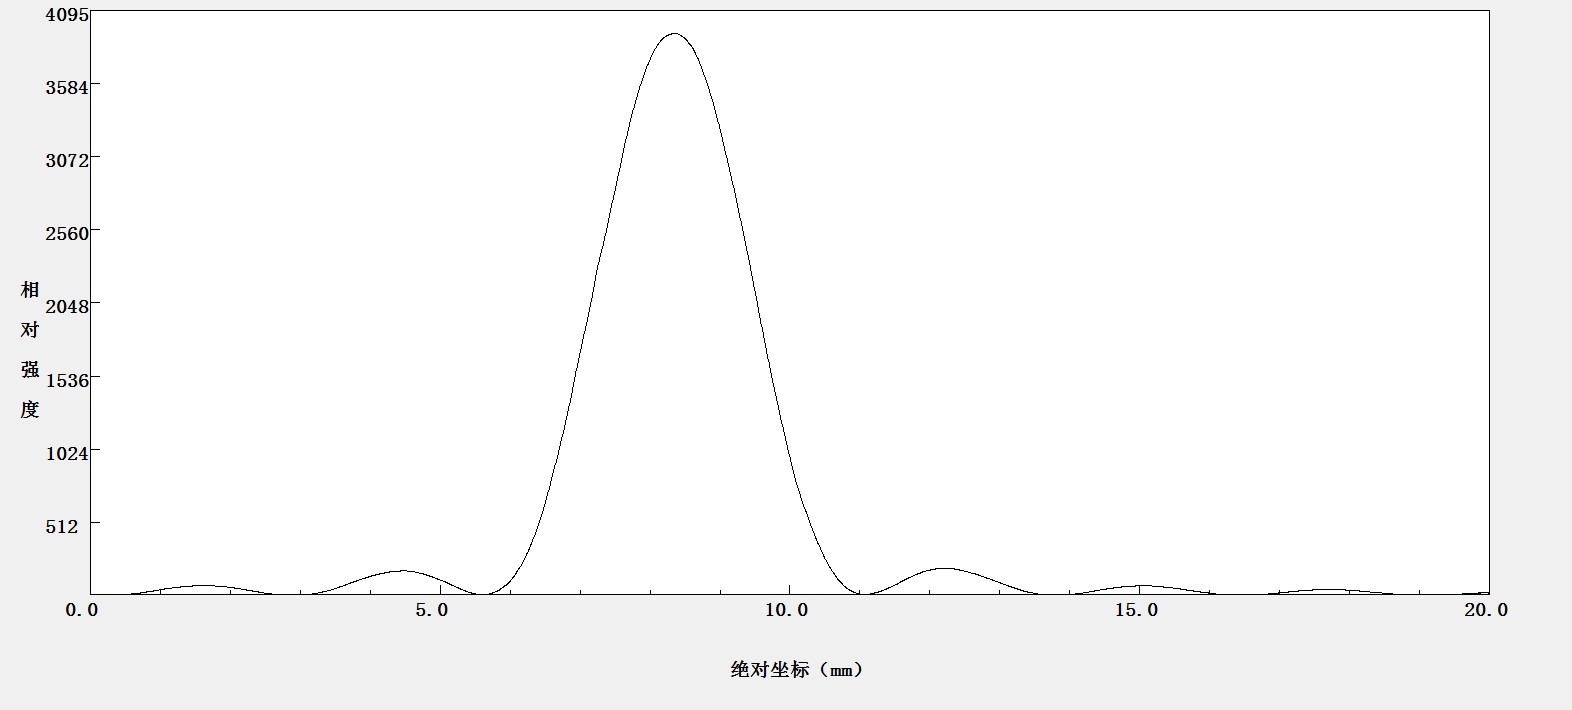
\includegraphics[width=\textwidth]{1.jpg}
        \label{fig:digit}
          
      \end{figure}

\subsubsection{计算}
利用数据处理软件,可以得到如下的数据表:
% Table generated by Excel2LaTeX from sheet '单缝'
\begin{table}[H]
    \centering
    \caption{光强测量之数据}
      \begin{tabular}{|c|c|c|c|c|c|}\hline
      花样名   &{零级主大值} &{左方次极大} &{右方次极大} &{左方零级暗纹} &{右方零级暗纹} \\ \hline
      位置$/mm$ &$x_0= 8.350$ &$x_1 =4.475$ & $x_2=12.195$ &$x_{01}= 5.605 $& $x_{02}=11.075$ \\\hline
      相对强度&$I_0=3934$  & $I_1=173$ & $I_2=191$ & $I_{01}=5$ & $I_{02}=7$\\\hline
      \end{tabular}%
    \label{tab:addlabel}%
  \end{table}%
  
  此外,需测量一些距离参数如下表:
  % Table generated by Excel2LaTeX from sheet '单缝'
\begin{table}[htbp]
  \centering
  \caption{光学元件距离}
    \begin{tabular}{|c|c|c|}\hline
    光学元件  & {探测器} & {单缝位置} \\ \hline
    位置$/cm$ & $z_0=14.88$ & $z_1=72.55$ \\\hline
    \end{tabular}%
  \label{tab:addlabel}%
\end{table}%



本实验中所用激光器为氦氖激光器,其波长$\lambda=632.8nm$。有远场条件$z>>\frac{\rho^2}{\lambda}$成立。

同时,其相对光强满足$$\frac{I_1+I_2}{2I_0}=4.6\%\in(4\%,5.5\%)$$
$$\frac{|I_1-I_2|}{(I_1+I_2)/2}=9.8\%<10\%$$

下进行计算:
\paragraph{利用一级级强计算缝宽}
根据公式
$$a=\frac{1.43\lambda}{\sin{\theta}}$$

并由$$\sin{\theta}\approx \frac{\Delta x}{z}$$

联立,并代入数据计算,得:

$$a=\frac{1.43 \times \lambda \times z}{\Delta x}=135.20(\mu m)$$


式中:$$\Delta x=|x_2-x_1|/2=3.860(mm)$$
$$z=|z_0-z_1|=57.67(cm)$$

由于$135.20\mbox{与参考值}133\mbox{相差小于}2\%$,故认为实验结果是可靠的。

下计算不确定度:

从计算公式出发,可看出共有三个参数,其中$$\lambda$$值可视为准确值(激光器产生)。从而有如下公式:
$$\frac{\sigma_a}a=\sqrt{(\frac{\sigma_x}{\Delta x})^2+(\frac{\sigma_z}z)^2}$$

又$$\sigma_x=\frac{e_x}{\sqrt{3}}=\frac{e_{x1}+e_{x2}}{\sqrt{3}}=$$
      \section{收获与感想}
      本次实验,是本学期的最后一个实验,而实验的内容,也是大家所常听闻的电路谐振。

      在进行实验的时候,我通过对$U_C$与$U$的观察,切身感受到了共振现象。而在计算中,也发现三种方法所得的$Q$值大致相等,也感受到理论的精妙。

      从实验中,我从将电路中电流信号,转变为串接电阻的电压信号这一设计,感受到了信号转换的重要性,这一点在过往的实验课程中也一再的强调。

      此外,在本次实验中,我也感受到了自己某些实验能力还有不足,例如电路接线,示波器的使用等,希望在以后的实验课程中,能够提高自己的实验能力。

\end{document} 